\Chapter{Instability in Current Mode Control}
\label{app:instability-cmc}
	Consider the waveform of steady state switch current as shown in figure \ref{fig:19} for a buck converter operating at duty cycle $D>0.5$. A small perturbation $\hat{i}_L(0)$ such that $|\hat{i}_L(0)| << |i_L(0)|$ is introduced in inductor current $i_L(t)$ which same as the switch current $i_s(t)$ at time $t=0$. During on time, the perturbed inductor current rises with slope of $m_1$ till time $(D+\hat{d})T_s$. At this instant, perturbed $i_L(t)=i_c(t)$ and the switch turns off. For the remainder of switching signal, $i_L(t)$ decreases with slope $-m_2$, and at $t=T_s$ the perturbation in inductor current is $\hat{i}_L(T_s)$. 
	\begin{figure}[H]
		\centering
		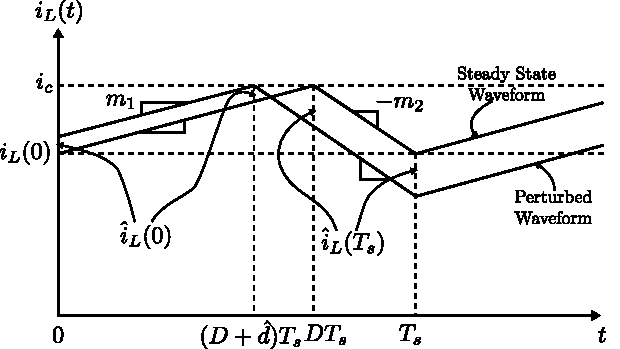
\includegraphics[width=0.8\textwidth]{wf-no-ramp}
		\caption{Inductor current in presence of disturbance}
		\label{fig:19}
	\end{figure}
	Figure \ref{fig:20} is the expanded view of perturbed and steady state inductor current between times $(D+\hat{d})T_s$ and $T_s$. Inductor current at time $t=0$ is given by
	\begin{equation*}
		i_L(0) = i_{L0} + \hat{i}_L(0)
	\end{equation*}
	The perturbation in inductor current at $t=0$ and $t=T_s$ are given by
	\begin{align}
		\hat{i}_L(0) &= -m_1\hat{d}T_s\\
		\hat{i}_L(T_s) &= m_2\hat{d}T_s\\
		\hat{i}_L(T_s) &= \hat{i}_L(0) \left( -\dfrac{m_2}{m_1} \right)
		\label{eq:5}
	\end{align}
	From relation governing slopes $m_1$ and $m_2$ in equation \eqref{eq:4},
	\begin{align}
		\hat{i}_L(T_s) &= \hat{i}_L(0) \left( -\dfrac{D}{1-D} \right)
		\label{eq:6}
	\end{align}
	At each cycle the perturbation will magnify by a factor of $\dfrac{D}{1-D}$, therefore, after $n$ such switching cycles, the perturbation in inductor current is
	\begin{equation}
		i_L(nT_s) = i_L(0)\left( -\dfrac{D}{1-D} \right)^n
		\label{eq:7}
	\end{equation}
	Thus, the magnification of initial perturbation depends on the duty ratio of the switch operation. If $D<0.5$, then the magnification factor $|\dfrac{D}{1-D}| < 1$, and any initial perturbations in the inductor or switch current will eventually die down. But, if $D>0.5$, then $|\dfrac{D}{1-D}| > 1$, the perturbations will only increase in magnitude with time, irrespective of the initial magnitude of the perturbation. Thus,
	\begin{align}
		|\hat{i}_L(nT_s)| \longrightarrow \left\{ 
		\parbox[]{2in}
		{$0 \quad \text{when} \quad \left|-\dfrac{D}{1-D}\right| < 1 $\\
		$\infty \quad \text{when} \quad \left|-\dfrac{D}{1-D}\right| > 1$}
		\right.
		\label{eq:8}
	\end{align}

	\begin{figure}[H]
		\begin{subfigure}{0.5\textwidth}
			\centering
			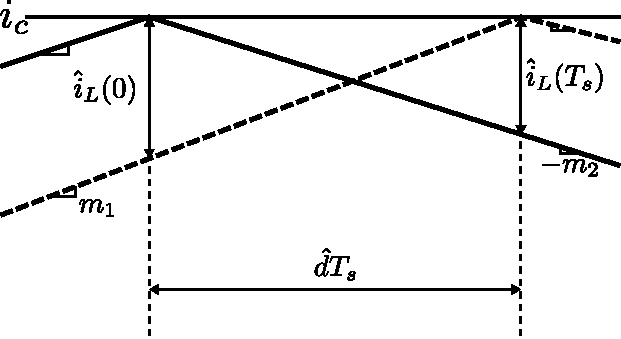
\includegraphics[width=\linewidth]{expanded-no-ramp}
			\caption{Perturbed inductor current}
			\label{fig:20}
		\end{subfigure}
		\begin{subfigure}{0.5\textwidth}
			\centering
			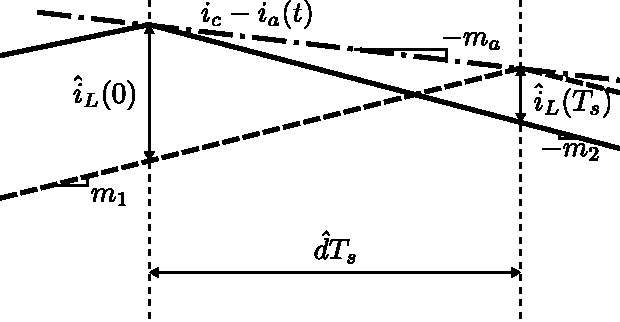
\includegraphics[width=\linewidth]{expanded-ramp}
			\caption{Perturbations with artificial ramp}
			\label{fig:23}
		\end{subfigure}
		\caption{Inductor current under disturbance}
	\end{figure}

	In this form, the satisfactory operation of converter is limited to a range $0 \leq D \leq 0.5$. To overcome this limitation, an artificial ramp $i_a(t)$ with slope $m_a$ and frequency equal to the switching frequency $F_s$ is added with the switch current as shown in figure \ref{fig:21}. Due to the addition of this ramp, the controller causes the switch to turn off when
	\begin{equation*}
		i_a(t) + i_L(t) = i_c
	\end{equation*}
	i.e.
	\begin{equation}
		i_L(t) = i_c - i_a(t)
		\label{eq:9}
	\end{equation}
	
	\begin{figure}[H]
		\centering
		
\includegraphics[width=0.8\textwidth]{current-mode-ramp}
		\caption{Block diagram of current mode control with artificial ramp compensation}
		\label{fig:21}
	\end{figure}

	\begin{figure}[H]
		\centering
		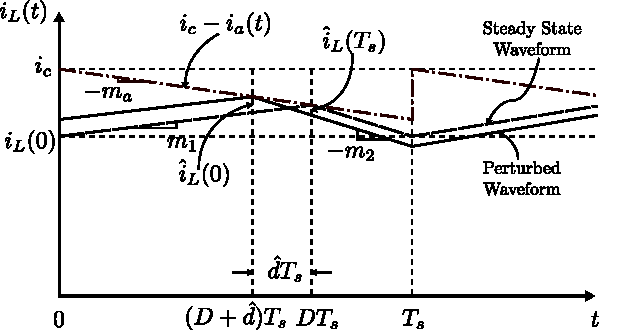
\includegraphics[width=0.8\textwidth]{wf-ramp}
		\caption{Inductor current with artificial ramp in presence of disturbance}
		\label{fig:22}
	\end{figure}

	Figure \ref{fig:22} shows the steady state and perturbed current waveforms for buck converter operating at duty $D>0.5$ in presence of initial perturbation $\hat{i}_L(0)$. From figure \ref{fig:23}, the initial disturbance in terms of slopes $m_1$ and $m_a$ is
	\begin{equation}
		\hat{i}_L(0) = -\hat{d}T_s(m_1+m_a)
		\label{eq:10}
	\end{equation}
	\begin{equation}
		\hat{i}_L(T_s) = -\hat{d}T_s(m_a-m_2)
		\label{eq:11}
	\end{equation}
	Therefore,
	\begin{equation}
		\hat{i}_L(T_s) = \hat{i}_L(0)\left(-\dfrac{m_2-m_a}{m_1+m_a} \right)
		\label{eq:12}
	\end{equation}

	The magnification in perturbation after $n$ switching cycles is
	Therefore,
	\begin{equation}
		\hat{i}_L(nT_s) = \hat{i}_L(0)\left(-\dfrac{m_2-m_a}{m_1+m_a} \right)^n
		\label{eq:13}
	\end{equation}

	When $n\longrightarrow \infty$,
	\begin{align}
		|\hat{i}_L(nT_s)| \longrightarrow \left\{ 
		\parbox[]{2in}
		{$0 \quad \text{when} \quad |\alpha| < 1 $\\
		$\infty \quad \text{when} \quad |\alpha| > 1$}
		\right.
		\label{eq:14}
	\end{align}
	where $$ \alpha = -\dfrac{m_2-m_a}{m_1+m_a} $$
	For stable operation of converter, the slope of the artificial ramp $m_a$ such that the magnification factor $|\alpha| < 1$. $\alpha$ from can be rearranged as
	\begin{equation}
		\alpha = -\dfrac{1-\dfrac{m_a}{m_2}}{\dfrac{1-D}{D}+\dfrac{m_a}{m_2}}
		\label{eq:15}
	\end{equation}

	If $m_a$ is chosen such that $m_a = \dfrac{1}{2}m_2$, then from equation \eqref{eq:15} $\alpha = -1$ at $D = 1$ and $|\alpha|<1$ for $0 \leq D < 1$. This is the minimum slope required for artificial ramp to stabilise the operation of converter over all operating duties. If $m_a$ is chosen such that $m_a = m_2$, then $\alpha$ is zero for all $D$. Therefore, $\hat{i}_L(T_s)$ is $0$ for any $\hat{i}_L(0)$. Thus, the system has finite settling time and removes any perturbation after one switching period $T_s$.